
% Copyright (c) 2015 - 2020 Mario Mlačak, mmlacak@gmail.com
% Licensed and published as Public Domain work.

% Nineteen chapter ====================================================
\chapter*{Nineteen}
\addcontentsline{toc}{chapter}{Nineteen}

\begin{flushright}
\parbox{0.8\textwidth}{
\emph{The truth is at the beginning of anything and its end are alike touching. \\
\hspace*{\fill}{\textperiodcentered \textperiodcentered \textperiodcentered \hspace*{0.2em} Yoshida Kenko} } }
\end{flushright}

\noindent
Nineteen is chess variant which is played on 18 x 18 board, with
light gold-yellow and white fields and gold-yellow and dark gray
pieces. In algebraic notation, columns are enumerated from 'a' to 'r',
and rows are enumerated from '1' to '18'. A new piece is introduced,
Star.

\clearpage % ..........................................................
% Star ****************************************************************

\section*{Star}
\addcontentsline{toc}{section}{Star}

% \vspace*{-1.3\baselineskip}
\noindent
\begin{wrapfigure}[11]{l}{0.4\textwidth}
\centering
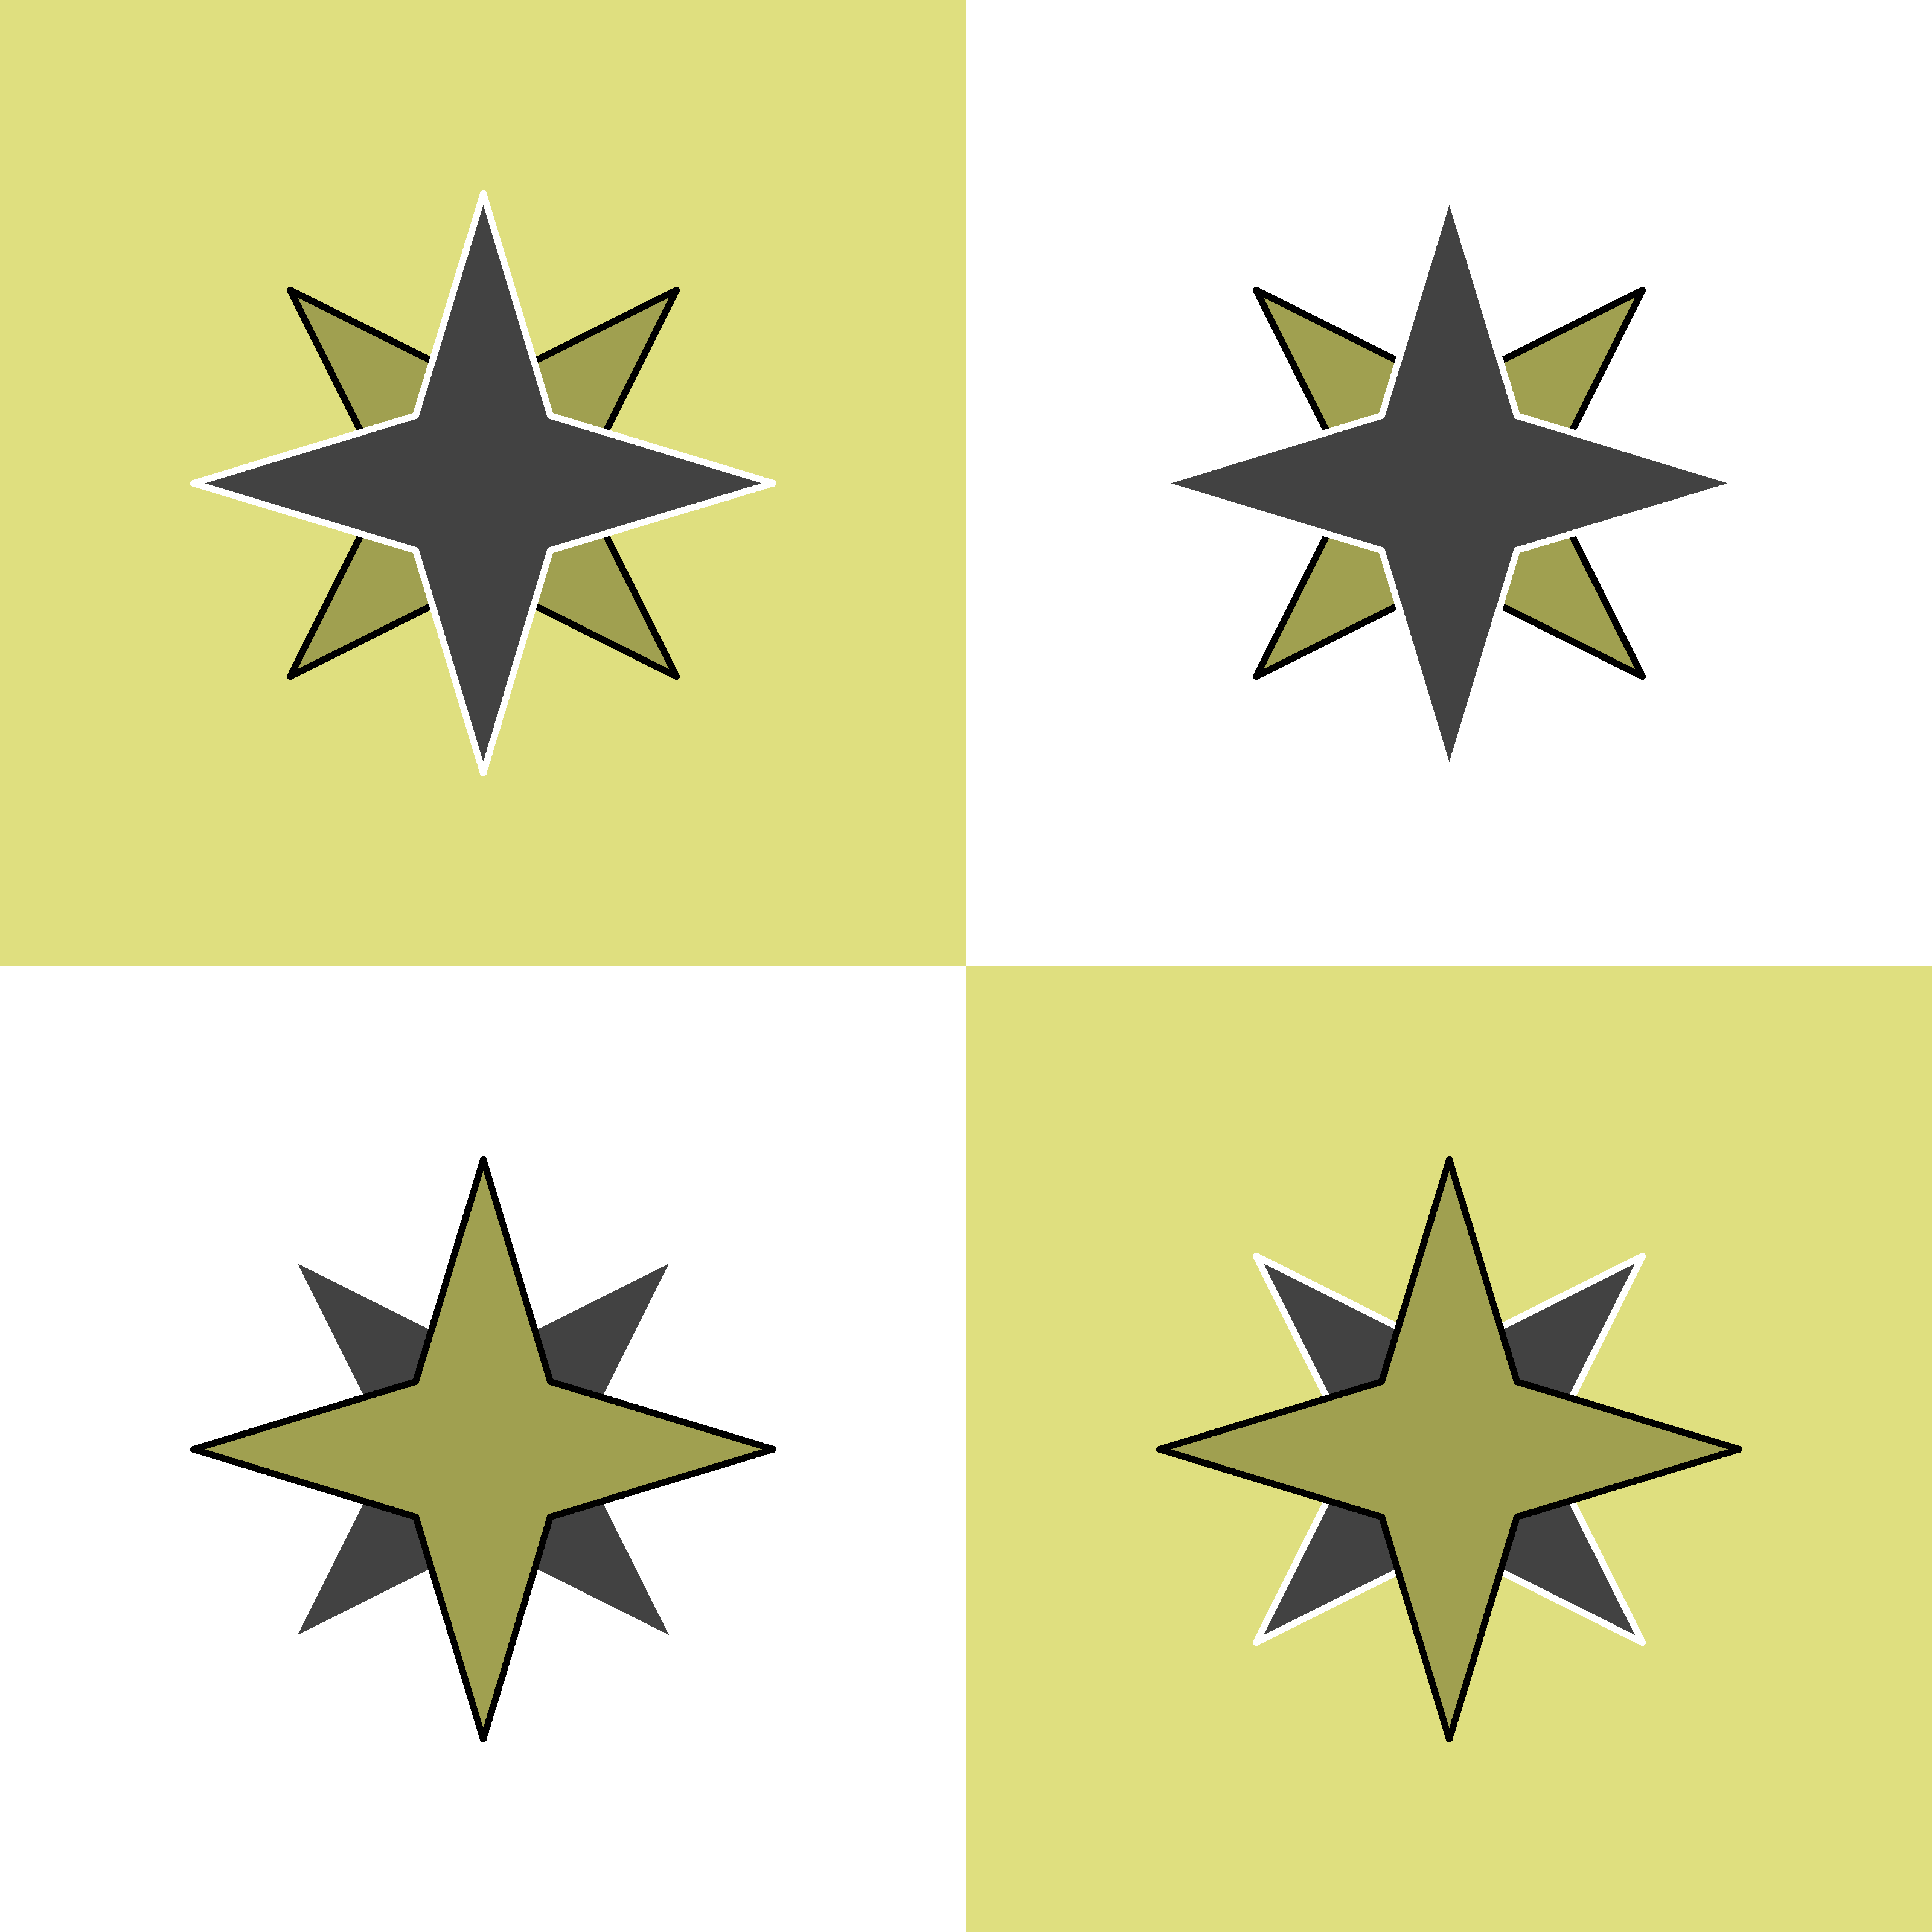
\includegraphics[width=0.4\textwidth, keepaspectratio=true]{pieces/11_star.png}
\caption{Star}
\label{fig:11_star}
\end{wrapfigure}
Star does not belong to any player, and can't be moved, activated, captured or converted by
either. Light Stars are positioned in lower left and upper right corners, dark Stars in lower
right and upper left corners.

Star is a teleporting piece. Teleportation is initiated by touching a field (or a Star) at
which it stands with a piece, using either normal or capturing step. Piece in question, if it's
not Wave, then reappears on any empty portal-field near Star in opposite color. Any momentum
carried is lost. Teleportation is not limited by matching colors of a piece and a Star, any
piece can use any Star to start teleporting.

Player initiating teleportation can choose which opposite color Star will be destination,
and at which empty portal-field piece will reappear. If there is no empty portal-field near
both Stars of opposite color, piece is removed from chessboard as if it has been captured.

If teleported piece is Wave, it continues movement from a field occupied by the other Star in
the same color. Wave retains all of momentum carried into teleportation. The way and direction
of movement of Wave is the same as before teleportation.

Kings cannot be teleported.
Pawns cannot be promoted to a Star.
In algebraic notation symbol for Star is 'T'.

\clearpage % ..........................................................

\subsection*{Portal-fields}
\addcontentsline{toc}{subsection}{Portal-fields}

\noindent
\begin{figure}[!h]
% \begin{figure}[!t]
\includegraphics[width=1.0\textwidth, keepaspectratio=true]{examples/12_n/scn_n_01_portal_fields.png}
\caption{Portal-fields}
\label{fig:scn_n_01_portal_fields}
% \centering
\end{figure}

Portal-fields are all fields immediately surrounding a particular field
horizontally, vertically and diagonally. They are the same as step-fields
of a King.

Since all Stars are pinned into the corners of a chessboard, there are always
exactly 3 portal-fields around each one.

\clearpage % ..........................................................
% Teleporting pieces ==================================================

\subsection*{Teleporting pieces}
\addcontentsline{toc}{subsection}{Teleporting pieces}

\noindent
\begin{figure}[!h]
% \begin{figure}[!t]
\includegraphics[width=1.0\textwidth, keepaspectratio=true]{examples/12_n/scn_n_02_teleport_init.png}
\caption{Teleportation start}
\label{fig:scn_n_02_teleport_init}
% \centering
\end{figure}

Light Bishop is about to teleport by diving into dark Star. Normaly, teleport
destination could be chosen among empty portal-fields of both light Stars.
Here, portal-field are all blocked, except field 1.

\clearpage % ..........................................................

\noindent
\begin{figure}[!h]
% \begin{figure}[!t]
\includegraphics[width=1.0\textwidth, keepaspectratio=true]{examples/12_n/scn_n_03_teleport_move_2.png}
\caption{Teleporting dark Rook}
\label{fig:scn_n_03_teleport_move_2}
% \centering
\end{figure}

While dark Wave (on field 1) could be activated by dark Rook in a normal,
non-teleporting ply, it cannot be activated by teleported dark Rook, because
dark Rook will have no momentum after teleportation. So, for teleporting dark
Rook all portal-fields around both light Stars are blocked, and so after
teleportation it will be removed from chessboard.

\clearpage % ..........................................................

\noindent
\begin{figure}[!h]
% \begin{figure}[!t]
\includegraphics[width=1.0\textwidth, keepaspectratio=true]{examples/12_n/scn_n_04_teleport_move_3.png}
\caption{Teleporting light}
\label{fig:scn_n_04_teleport_move_3}
% \centering
\end{figure}

Wave can reach a Star and start teleporting even if activating piece (here,
Pegasus) would be blocked.

\clearpage % ..........................................................

\noindent
\begin{figure}[!h]
% \begin{figure}[!t]
\includegraphics[width=1.0\textwidth, keepaspectratio=true]{examples/12_n/scn_n_05_teleport_end.png}
\caption{Teleportation end}
\label{fig:scn_n_05_teleport_end}
% \centering
\end{figure}

Teleported Wave emerges from the other Star in the same color as the starting one.
Wave has to continue movement in the same direction as it did before teleportation,
direction cannot be changed. Wave also retains momentum it had before teleportation,
so here it can activate Pyramid, or
\hyperref[fig:scn_mv_18_activating_rush_pawn_init]{rush light Pawn for 2 fields}.

\clearpage % ..........................................................

\noindent
\begin{figure}[!h]
% \begin{figure}[!t]
\includegraphics[width=1.0\textwidth, keepaspectratio=true]{examples/12_n/scn_n_06_teleport_wave_blocked.png}
\caption{Teleported Wave blocked}
\label{fig:scn_n_06_teleport_wave_blocked}
% \centering
\end{figure}

If teleported Wave has all of its' step-fields blocked (here, by dark Pawns), it is
removed from chessboard, just like any other
\hyperref[fig:scn_n_03_teleport_move_2]{teleported piece which has all portal-fields blocked}.

\clearpage % ..........................................................
% Teleporting Wave ----------------------------------------------------

\subsubsection*{Teleporting Wave}
\addcontentsline{toc}{subsubsection}{Teleporting Wave}

\vspace*{-1.2\baselineskip}
\noindent
\begin{figure}[!h]
% \begin{figure}[!t]
\includegraphics[width=1.0\textwidth, keepaspectratio=true]{examples/12_n/scn_n_07_teleport_wave_init.png}
\caption{Wave out-of-board before teleportation}
\label{fig:scn_n_07_teleport_wave_init}
% \centering
\end{figure}

Here, light grey fields are virtual fields extending existing chessboard.
\hyperref[fig:scn_mv_24_wave_activation_by_unicorn]{Wave activated by Unicorn}
has to choose 2 different steps at the beginning of its’ movement, and follow
them for the remainder of a ply. Wave's movement is legal as long as its’
\hyperref[fig:scn_mv_26_wave_off_board]{ply ends on a chessboard}. So, light
Wave can reach light Star and start teleporting, even though it stepped
outside of a board.

\clearpage % ..........................................................

\noindent
\begin{figure}[!h]
% \begin{figure}[!t]
\includegraphics[width=1.0\textwidth, keepaspectratio=true]{examples/12_n/scn_n_08_teleport_wave_end.png}
\caption{Wave teleported}
\label{fig:scn_n_08_teleport_wave_end}
% \centering
\end{figure}

Teleported Wave has to continue its' movement performing the same step(s) as
before teleportation. That means, teleported Wave has to continue alternating
between 2 initially chosen steps, according to a color of a current field. So,
emerging step (here, long jump) is different from a step starting teleportation
(short jump).

\clearpage % ..........................................................

\noindent
\begin{figure}[!h]
% \begin{figure}[!t]
\includegraphics[width=1.0\textwidth, keepaspectratio=true]{examples/12_n/scn_n_09_teleport_wave_2_init.png}
\caption{Wave before teleportation}
\label{fig:scn_n_09_teleport_wave_2_init}
% \centering
\end{figure}

Similar example as previous, with dark Wave which has the same steps (short,
long jump) over the same colored fields (dark, light fields) switched. So,
teleporting step is also different (here, long jump) from previous example
(short jump).

\clearpage % ..........................................................

\noindent
\begin{figure}[!h]
% \begin{figure}[!t]
\includegraphics[width=1.0\textwidth, keepaspectratio=true]{examples/12_n/scn_n_10_teleport_wave_2_end.png}
\caption{Wave out-of-board after teleportation}
\label{fig:scn_n_10_teleport_wave_2_end}
% \centering
\end{figure}

\hyperref[fig:scn_n_08_teleport_wave_end]{Again},
teleported Wave has to continue alternating between 2 initially chosen steps,
according to a color of a current field, i.e. color of starting field of each
step. Wave's movement is legal as long as its’
\hyperref[fig:scn_mv_26_wave_off_board]{ply ends on a chessboard}. So, dark
Wave can e.g. activate dark Pawn (with 1 momentum carried through teleportation),
even though it stepped outside of a board.

% ---------------------------------------------------- Teleporting Wave
\clearpage % ..........................................................
% Teleporting Pawn ----------------------------------------------------

\huge{}
TODO :: remove rushing of converted Pawn\
DONT :: remove definition of piece, figure, Pawn, rush rows
\normalsize{}

\clearpage % ..........................................................

\subsubsection*{Teleporting Pawn}
\addcontentsline{toc}{subsubsection}{Teleporting Pawn}

\vspace*{-1.4\baselineskip}
\noindent
\begin{figure}[!h]
% \begin{figure}[!t]
\includegraphics[width=1.0\textwidth, keepaspectratio=true]{examples/12_n/scn_n_11_teleport_pawns_init.png}
\caption{Pawn teleporting on step-field}
\label{fig:scn_n_11_teleport_pawns_init}
% \centering
\end{figure}

All pieces can access a Star on own step- or capture-field. So, light Pawn in
the same column as dark Star (here, a) can step into it, and teleport away. If
destination Star is on
\hyperref[sec:Definitions/Sides of a chessboard]{opponent's side of a board},
teleported Pawn is tagged for
promotion (green, blue fields). If destination portal-field is on opponent's
\hyperref[sec:Age of Aquarius/Promotion/Figure, Pawn, piece and rush rows]{figure row}
(blue), player can choose between promoting Pawn outright, or keeping it tagged
for promotion.

\clearpage % ..........................................................

\noindent
\begin{figure}[!h]
% \begin{figure}[!t]
\includegraphics[width=1.0\textwidth, keepaspectratio=true]{examples/12_n/scn_n_12_teleport_pawns_step_1.png}
\caption{Pawn teleporting on capture-field}
\label{fig:scn_n_12_teleport_pawns_step_1}
% \centering
\end{figure}

Pawn can also dive into a Star located at its' capture-field, and teleport away.
If destination Star is on
\hyperref[sec:Definitions/Sides of a chessboard]{own side of a board} (portal-fields
4, 5, 6), teleported Pawn loses options to promote. Teleported Pawn gains opportunity
to rush on an initial move, similar to
\hyperref[fig:scn_aoa_13_opponents_pawn_converted]{Pawns converted on own piece rows}.

\clearpage % ..........................................................

\noindent
\begin{figure}[!h]
% \begin{figure}[!t]
\includegraphics[width=1.0\textwidth, keepaspectratio=true]{examples/12_n/scn_n_13_teleport_pawns_end.png}
\caption{Pawn teleporting end}
\label{fig:scn_n_13_teleport_pawns_end}
% \centering
\end{figure}

Light Pawn teleported onto own side of chessboard can now rush up to (and including)
the last row on own side of chessboard. In this variant that means, on an initial
move Pawn can rush for
\hyperref[fig:12_nineteen_en_passant]{up to 7 fields from own Pawns row}
(fields 4, 5), and up to 8 fields from own figure row (field 6).

% ---------------------------------------------------- Teleporting Pawn
\clearpage % ..........................................................

\subsubsection*{Teleporting Bishop}
\addcontentsline{toc}{subsubsection}{Teleporting Bishop}

\vspace*{-1.1\baselineskip}
\noindent
\begin{figure}[!h]
% \begin{figure}[!t]
\includegraphics[width=1.0\textwidth, keepaspectratio=true]{examples/12_n/scn_n_14_teleport_bishop.png}
\caption{Bishop teleportation}
\label{fig:scn_n_14_teleport_bishop}
% \centering
\end{figure}

Teleporting Bishop, like any other piece, can choose any empty portal-field
around opposite-color Star as a destination, regardless of a field's color.
Teleporting to a field in a different color changes (color of) accessible
fields for teleported Bishop, for the remainder of a game. Here, such
color-changing portal-fields are enumerated, 1 and 2.

% ================================================== Teleporting pieces
% **************************************************************** Star
\clearpage % ..........................................................

\section*{Promotion}
\addcontentsline{toc}{section}{Promotion}

Promotion is non enforced, delayed variety, i.e. it's the same as in
\hyperref[sec:Age of Aquarius/Promotion]{previous chess variant}, Age of Aquarius.

Again, Pawns cannot be promoted to a Star.

Additionaly, promotion in this variant is monogamous.
Only one Queen in the same color can be present on chessboard at any given time.

\clearpage % ..........................................................

\section*{Pawn ranks, rows}
\addcontentsline{toc}{section}{Pawn ranks, rows}

\vspace*{-1.1\baselineskip}
\noindent
\begin{figure}[!h]
% \begin{figure}[!t]
\includegraphics[width=1.0\textwidth, keepaspectratio=true]{examples/12_n/scn_n_15_pawn_ranks.png}
\caption{Pawn rows}
\label{fig:scn_n_15_pawn_ranks}
% \centering
\end{figure}

In this variant, an additional rank of light (blue arrow) and dark (red) Pawns has
been added to \hyperref[fig:12_nineteen]{initial setup}. Ranks of Pawns are enumerated
starting with one closest to opponent; the closest rank being the first one (blue,
red arrows), while the standard rank of Pawns is the second rank (green, grey).

\clearpage % ..........................................................

\huge{}
TODO :: remove rushing of converted Pawn\
DONT :: remove definition of piece, figure, Pawn, rush rows
\normalsize{}

\clearpage % ..........................................................

\section*{Rush, en passant}
\addcontentsline{toc}{section}{Rush, en passant}

\noindent
\begin{wrapfigure}[12]{l}{0.4\textwidth}
\centering
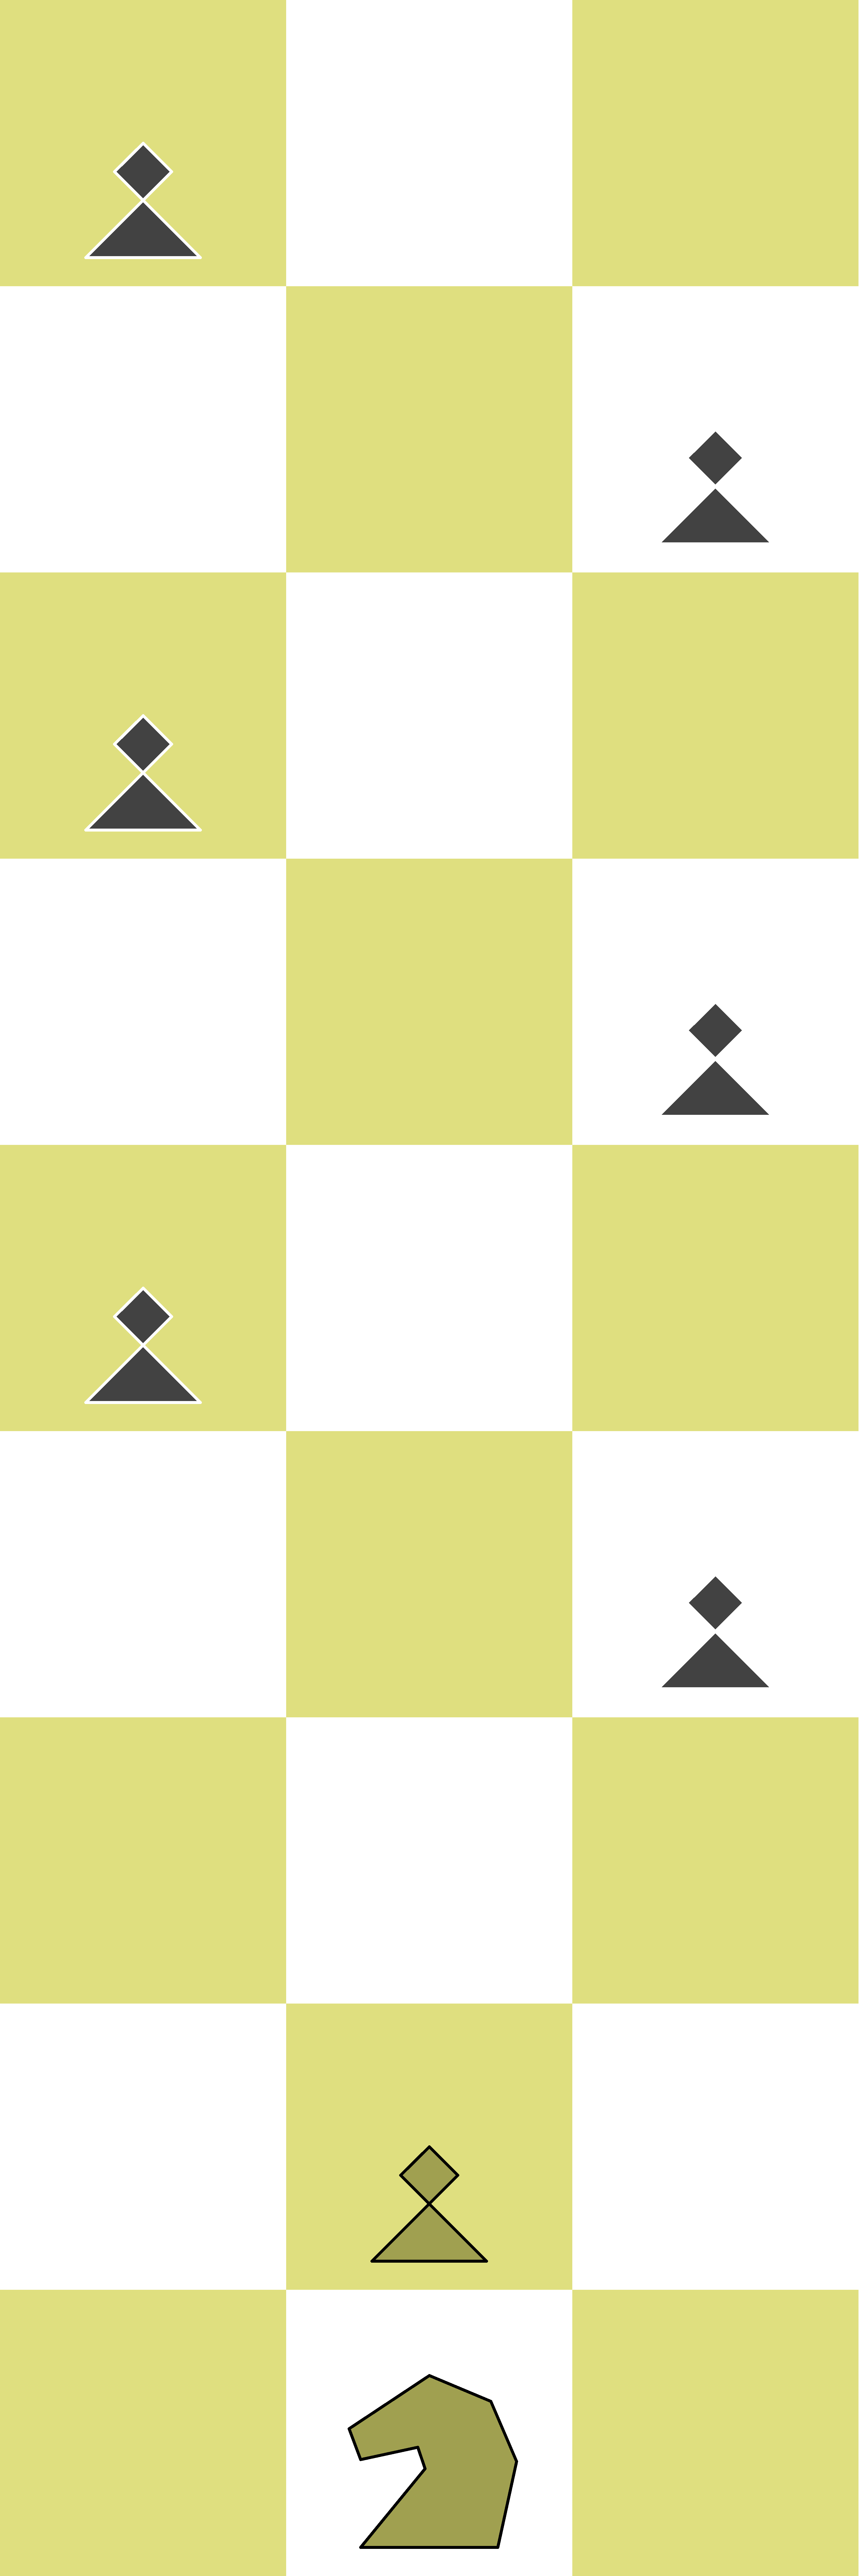
\includegraphics[width=0.388888889\textwidth, keepaspectratio=true]{en_passants/12_nineteen_en_passant.png}
\caption{En passant}
\label{fig:12_nineteen_en_passant}
\end{wrapfigure}
Rush and en passant are very similar to those in Classic Chess.

Pawns from both ranks can be rushed, up to the other end of
\hyperref[sec:Definitions/Sides of a chessboard]{own side of the chessboard}.

In this variant, Pawns in the first row (A) can be rushed for up to 6 fields,
while those in second row (B) can go up to 7 fields forward.

Opponent's Pawns converted in either own Pawns or figure rows,
\hyperref[fig:scn_aoa_11_opponents_pawn_conv_init]{like in previous variants},
can be rushed up to and including the furthest own row of chessboard.

So, opponent's Pawns converted in own Pawns rows can be rushed for up to 6 or
7 fields, depending if place of conversion were the first or the second Pawns
row, respectively.
Opponent's Pawns converted in own figure row can be rushed up to 8 fields.

Option to rush converted opponent's Pawns, just like for initially own Pawns,
is valid only for their very first move.

\clearpage % ..........................................................

\section*{Castling}
\addcontentsline{toc}{section}{Castling}

Castling is the same as in Classical Chess, only difference is that King can move between 2 and 6 fields across.
All other constraints from Classical Chess still applies.

\noindent
\begin{figure}[!h]
% \begin{figure}[!t]
\includegraphics[width=1.0\textwidth, keepaspectratio=true]{castlings/12_n/nineteen_castling.png}
\caption{Castling}
\label{fig:nineteen_castling}
% \centering
\end{figure}

In example above, all valid King's castling moves are numbered.

\noindent
\begin{figure}[!h]
% \begin{figure}[!t]
\includegraphics[width=1.0\textwidth, keepaspectratio=true]{castlings/12_n/nineteen_castling_left_05.png}
\caption{Castling long left}
\label{fig:nineteen_castling_left_05}
% \centering
\end{figure}

In this example King was castling long to the left. Initial King's position is marked with "K".
After castling is finished, left Rook ends up at field immediately right to the King.

\clearpage % ..........................................................

\section*{Initial setup}
\addcontentsline{toc}{section}{Initial setup}

Stars are positioned in very corners of chessboard, light Stars in lower left and upper right
corners, dark Stars in lower right and upper left corners. Additional rank of light and dark
Pawns has been added. All other figures are also repositioned.

\noindent
% \begin{figure}[t]
\begin{figure}[h]
\includegraphics[width=1.0\textwidth, keepaspectratio=true]{boards/12_nineteen.png}
\caption{Nineteen board}
\label{fig:12_nineteen}
% \centering
\end{figure}

\clearpage % ..........................................................
% ==================================================== Nineteen chapter
